\setcounter{subsection}{8}

\subsection{Арифметичность предикатов «n — степень шестёрки» и $n = 2^k$}

\textbf{Опр} Предикат P: $\mathbb {N} \rightarrow \{0,1\}$ называется \textit{арифметичным}, если он выразим в стандартной интерпретации арифметики $\{\mathbb {N}, +,*,=\}$. Функция $f: \mathbb{N}^k \rightarrow \mathbb{N}$ называется \textit{арифметичной}, если арифметичен предикат $P_{f}: \mathbb{N}^{k+1} \rightarrow \{0,1\}$, где $P_f(x,y) = 1 \leftrightarrow f(x) = y$
\\
\\
\textbf{Степень шестерки}
\\
Степень шестерки можно выразить с использованием квантора по конечному множеству\\
    $\exists D (x \in D \wedge \forall y \in D (y = 1 \vee (y \ \vdots \ 6 \wedge \frac{y}{6} \in D)))$ \\ У нас есть $x, \frac{x}{6}, \frac{x}{36}, \frac{x}{216}, ..., 1$. Этакий мешок с числами. И если в нем есть х, то есть и $\frac{x}{6}$ и т.д., а остановиться это все может только на единице. Соответственно, если x - не степень шестерки, то возникнет не единица, и оба условия будут нарушены.
    \\
    \\
    Через обычные предикаты эта функция выражается с помощью кодирования Смаллиана. Оно лучше применимо для описания конечных множеств. В чем суть:
    \\
    Берем и вводим предикат $S(a,b,x)$, которые отвечает следующим свойствам:
    \begin{itemize}
        \item [1] $\forall a,b\{x: S(a,b,x) = 1\}$ - конечно
        \item[2] Для любого конечного S найдутся такие a и b, что $S = \{x: S(a,b,x) = 1\}$
    \end{itemize}
    Теперь записанную нами формулу $\exists D .... x \in D....$ можно переписать следующим образом:\\
    $\exists a,\exists b (S(a,b,x) \wedge \forall y(S(a,b,y) \rightarrow (y = 1 \vee(y \ \vdots \ 6 \wedge \exists z(y = 6*z \wedge S(a,b,z))))))$ \\
    Что поменялось? Заменили $\exists D$ на $\exists a, \exists b$. И $x \in D$ на $S(a,b,x)$, получили формулу первого порядка\\\\
\textbf{Степень двойки}\\
$x = 2^k $ можно выразить с использованием квантора по конечной последовательности\\
$\exists \{a_i\} (a_0 = 1 \wedge a_k = x \wedge \forall i \in [0;k-1] \ a_{i+1} = a*a_i)$
\\
\\
Через обычные предикаты это выражается с использованием $\beta$-функции Гёделя. 
\\
Тут вводится арифметическая функция $\beta(a,b,i)$ со следующим свойством:
\begin{itemize}
    \item[] $\forall [x_0, ..., x_n]$ найдутся такие a,b, что $\forall i \in [0,n] \ x_i = \beta(a,b,i)$
\end{itemize}
Теперь в формуле, которая имеет вид $\exists \{x_i\} ......x_j......$ можно заменить на такую: $\exists a \exists b ......\beta(a,b,j)......$
\\
\\
Применим полученные знания к нашему предикату и получим:\\
$x = 2^k \Longleftrightarrow \exists a,b \ (\beta(a,b,0) = 1 \wedge \beta(a,b,k) = x \wedge \forall i \in [0,..., k-1] \ \beta(a,b,i+1) = 2*\beta(a,b,i) $


\subsection{Вывод коммутативности сложения в арифметике Пеано}
Хотим получить: $\forall x \forall y x+y = y+x$ \\
Будем доказывать в три этапа \\

\begin{center}
    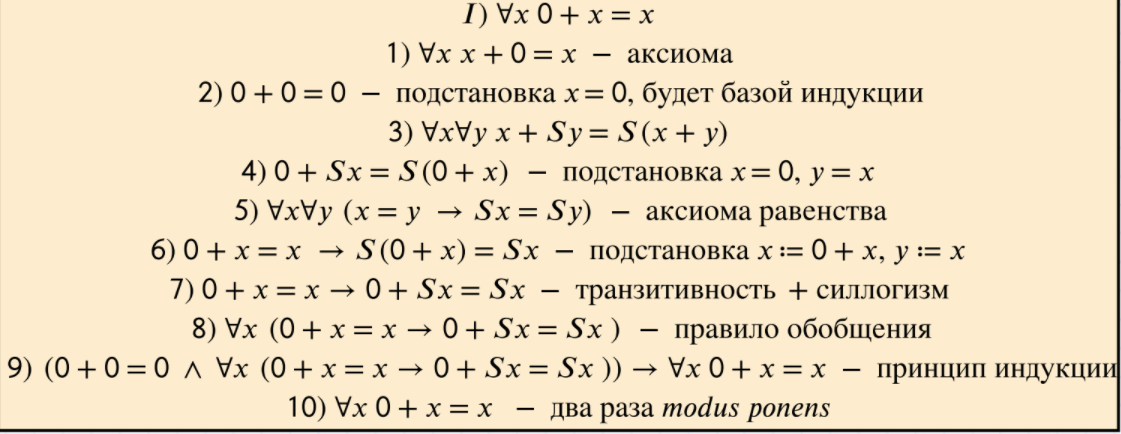
\includegraphics[width=9cm,height = 4.5cm]{images/1.9-1.12_m101.PNG}

    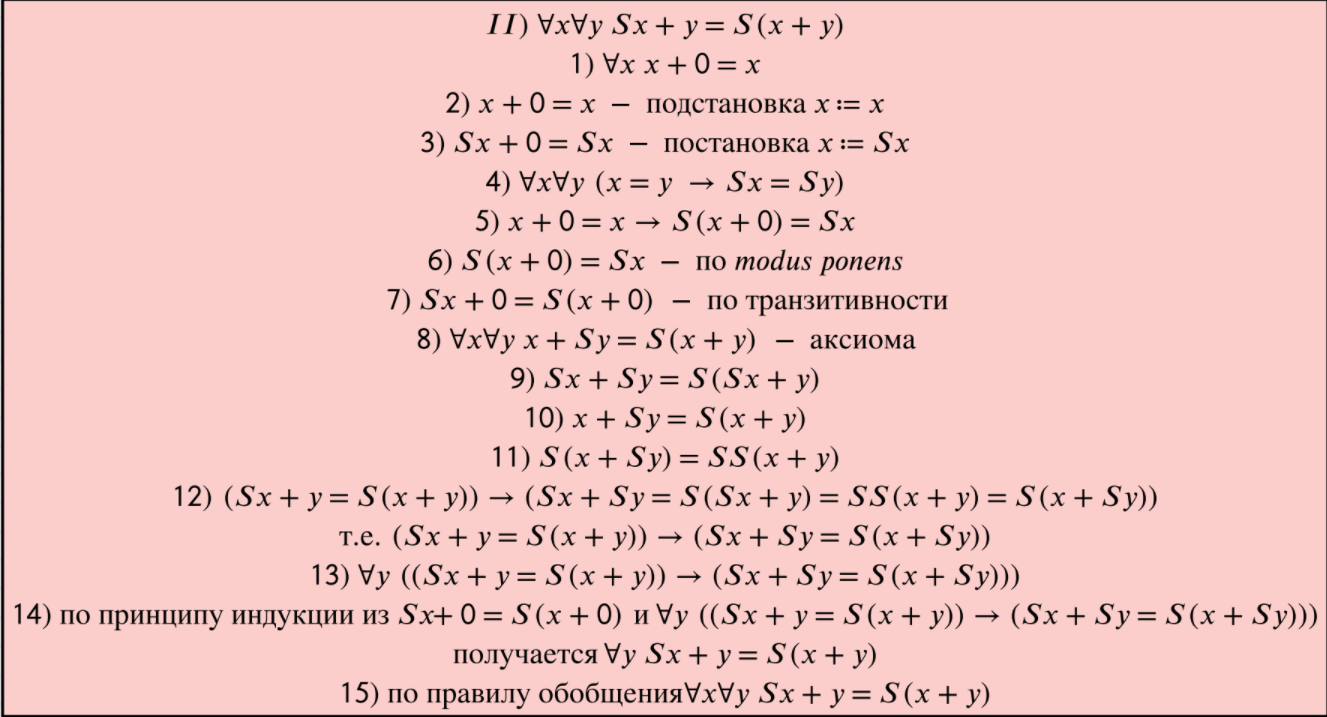
\includegraphics[width=9.8cm,height = 6cm]{images/1.9-1.12_m102.PNG}

    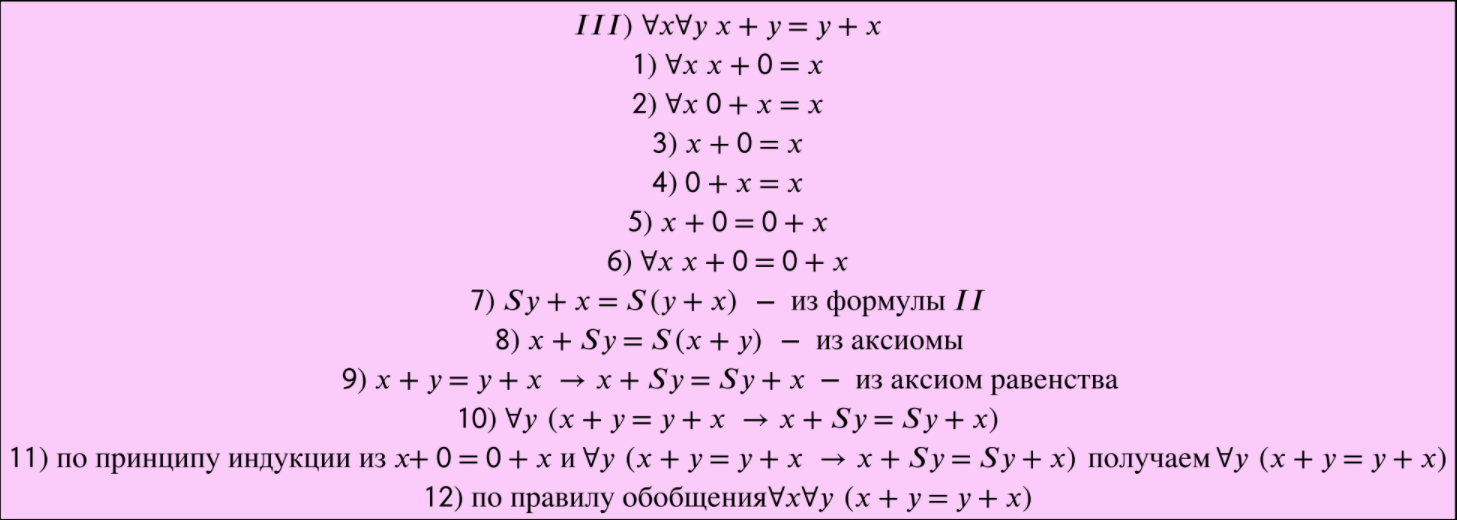
\includegraphics[width=15cm, height = 6cm]{images/1.9-1.12_m103.PNG}
\end{center}

\subsection{Множество замкнутых формул, истинных в $\mathbb N$, неперечислимо}

\textbf{Опр} Множество A $\subset \mathbb{N}^k$ называется \textit{арифметическим}, если существует арифметическая формула $\alpha$ с параметрами $x_1, . . . , x_k$, которая его представляет в следующем смысле: $<n_1, . . . , n_k>$ принадлежит множеству A тогда и только тогда, когда формула $\alpha$ истинна при значениях параметров $x_1 = n_1, . . . , x_k = n_k$.
\\
\\
Любое перечислимое множество арифметично
\\
\\
\textbf{Лемма1}\\
Всякое арифметическое множество лежит в классе $\Sigma_n$ или $\Pi_n$ для некоторого n (и, естественно, для всех больших n).
\\
$\blacktriangle$ Формулу, задающую арифметическое множество, приведём к предварённой нормальной форме (вынеся кванторы наружу). Ясно, что бескванторная часть задаёт разрешимое множество, поэтому исходное множество принадлежит какому-то из классов $\Sigma_n$ или $\Pi_n$. Можно и не использовать предварённой нормальной формы, а применить индукцию по длине формулы и сослаться на то, что пересечение, объединение и дополнение, а также проекция не выводят за пределы арифметической иерархии (объединения всех классов $\Sigma_n$ и $\Pi_n$). $\blacksquare$
\\
\\
Рассмотрим теперь множество T, элементами которого являются
все истинные арифметические формулы без параметров (точнее, их номера в какой-то вычислимой нумерации всех формул — это значит, что по формуле можно алгоритмически получить её номер и наоборот).
\\
\\
\textbf{Лемма2}\\ Любое арифметическое множество m-сводится к множеству T.\\
$\blacktriangle$ Пусть A — произвольное арифметическое множество. Пусть $\alpha$(x) — формула с одной переменной, которая выражает принадлежность множеству A. Это означает, что $\alpha$(n) истинно при тех и только тех n, которые принадлежат A.
Тогда вычислимая функция n $\rightarrow$ (номер формулы, которая является
результатом подстановки константы n в $\alpha$(x)) m-сводит A к T. $\blacksquare$
\\
\subsection{Первая теорема Гёделя о неполноте. Теорема Тарского}

\textbf{Теорема Тарского}\\
Истинность арифметической формулы нельзя выразить арифметическим выражением. То есть не существует формулы True(x), которая истинна тогда и только тогда, когда формула с номером х истинна. (Множество T не арифметично.)
\\
$\blacktriangle$ Если бы T было арифметическим, то оно лежало бы в некотором конкретном классе . Поскольку всякое арифметическое множество сводится к T, то все арифметические множества лежали бы в этом классе. Но мы знаем, что множества из более высоких классов иерархии тоже арифметичны, но в $\Sigma_n$ не лежат.$\blacksquare$
\\
\\
\textbf{ Первая теорема
Гёделя о неполноте}\\
Множество T арифметических истин неперечислимо.\\
$\blacktriangle$ Это следует из того, что если бы Т было перечислимо, оно было бы арифметично, что противоречит теореме Тарского $\blacksquare$ 
\\
\\
\textbf{Множество замкнутых формул, истинных в N, неперечислимо } \\
Если множество перечислимо, то оно лежит в арифметической иерархии, что противоречит теореме Тарского